\textbf{\uline{Exemplo 08:}}
	\begin{center}
        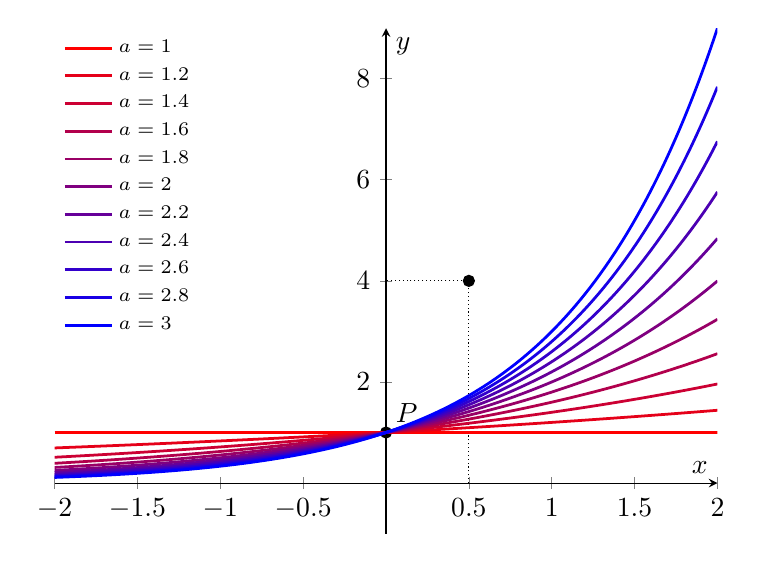
\begin{tikzpicture}
        	\begin{axis}[
        		xlabel=$x$,
        		ylabel=$y$,
        		width=10cm,
        		height=8cm,
        		axis lines = middle,
        		xmin=-2,
        		xmax=2,
        		ymin=-1,
        		%ymax=6000,
        		y tick label style={/pgf/number format/.cd,
        			set thousands separator={.}
        		},
        		legend style = {
        			at={(0,1)},
        			anchor=north west,
        			font=\scriptsize,
        			legend columns=1,
        			legend cell align=left,
        			draw=none
        		},
        		]
        		\draw[fill] (axis cs: 0,1) circle (2pt);
        		\node[anchor=south west] at (axis cs: 0,1) {$P$};
        		\draw[densely dotted] (axis cs: 0.5,0) -- (axis cs: 0.5,4) -- (axis cs: 0,4);
        		\draw[fill] (axis cs: 0.5,4) circle (2pt);
        		%
        		\foreach \a [count=\i] in {1,1.2,...,3}{
        			\edef\grafico{\noexpand
        				\addplot[blue!\fpeval{(\i-1)*100/10}!red,line width=1pt,smooth,samples=100,domain=-2:2] ({x},{\a^x});
        			}
        			\addlegendentryexpanded{$a=\fpeval{round(\a,1)}$}
        			\grafico
        		}
        	\end{axis}    
        \end{tikzpicture}
	\end{center}